\chapter{Auswertung}
\section{Auswertung der subjektiven Beobachtungen}
Im folgenden Abschnitt wird die Auswertung der im vorherigen Kapitel beschriebenen Beobachtungen durchgeführt.
\subsection{Problemstellung}
Nach Abschluss der Beobachtungsphase der Kinder musste nun eine Grundlage geschaffen werden, so dass die Daten, die dabei gesammelt wurden, miteinander vergleichbar werden. Durch die subjektive Beobachtungen der Autoren ist die Vergleichbarkeit nicht gegeben. Daher wurde für die Studienarbeit eine Metrik geschaffen, deren Ziel es war, aus subjektiven Bewertungen Werte zu erhalten, mit welchen besser gerechnet und verglichen werden kann.
\subsection{Entwicklung einer Metrik}
Nachdem alle Daten der Kinder erfasst wurden, sowohl die der Kinder an der \acrshort{dhbw} Karlsruhe als auch an der \acrlong{guc}, wurden alle während der Beobachtung verfassten Formulierungen gesammelt. Dies wurde gemacht, um einen Überblick darüber zu gewinnen, welches Spektrum die Aussagen der Beobachter bildeten. Um aus diesen Formulierungen ein mathematisches Spektrum zu erhalten, mussten zwei Kernfragen beantwortet werden.\\
Zuerst musste geklärt werden, wie feinstufig das Spektrum sein musste. Dies hing davon ab, wie viele verschiedene Formulierungen es bei den einzelnen Antworten gab. Häufig waren jedoch die Antworten sehr überschaubar, oftmals wurde nur ein einzelnes ´"yes'" oder `"no'" in den Beobachtungsbögen eingetragen, so dass die Skala, mit der später die Formulierungen in Zahlenwerte umgewandelt werden sollte, nicht sehr fein sein musste. Für die Skala wurde deshalb ein fünfstufiges System definiert. Die Skala beinhaltete einen positiven und einen negativen Teil, welche beide aus je zwei Stufen bestanden. Für die Anschaulichkeit wurde eine zweite Skala geschaffen, so dass es einfacher war, die Werte einzuteilen. Die fünf Stufen, die die Skala zur Anschauung bildeten, waren folgende: --,-,0,+,++. Die Stufe, welche als -- bezeichnet wurde, steht ganz links auf der Skala und bildet damit den schlechtesten Wert. Auf der positiven Seite bildet die Stufe mit der Bezeichnung ++ den höchsten Wert. Mit diesen Bezeichnungen ist es nun möglich, Formulierungen einzuordnen.\\
Da mit diesen Bezeichnungen jedoch noch keine arithmetischen Operationen durchgeführt werden konnte, wurde nun eine zweite fünfstufige Skala definiert. Deren Minimum ist bei 0, was auf der Anschauungs-Skala der Bezeichnung -- entspricht. Das Maximum der Skala liegt bei 4 und ist das Gegenstück zu der Stufe mit der Bezeichnung ++ auf der Anschauungs-Skala. Nachdem die Formulierungen nun in Stufen eingeteilt wurden, konnte mithilfe dieser neuen Skala aus den Beobachtungen Daten gewonnen werden, mit denen nun Vergleiche möglich sind.\\

Die zweite Kernfrage, die sich gestellt hatte, war welche Formulierung in welche Stufe eingeordnet werden muss. Hierfür wurde noch einmal das Spektrum der Beobachtungen analysiert. Durch die bereits erwähnte Häufigkeit der Formulierung `"yes'" wurde diese als Nullpunkt der Skala definiert. Für das linke Ende der Skala wurde `"no'" definiert. Auf der rechten Seite der Skala wurde keine Formulierung definiert, welche das Maximum darstellte.\\
Bei der Einteilung der restlichen Formulierungen wurde danach geschaut, ob eine Formulierung inhaltlich das Kind besser oder schlechter bewerteten als `"yes'". Sollte es zwischen `"no'" und `"yes'" liegen, so wurde es mit einer Eins bewertet, sollte es besser sein wurde, je nach dem wie sehr positiv die Formulierung war, mit einer Drei oder der Maximalpunktzahl Vier bewertet.\\

Die definierte Skalen sind in der untenstehenden Tabelle definiert. Das Bilden der Skala wurde von einer Studentin der \acrlong{guc} übernommen, welche nur die ihr zur Verfügung gestellten Bewertungsbögen als Grundlage dafür hatte.

\begin{table}[H]
	\centering
	\begin{tabular}{|c|c|c|c|c|}
		\hline
		-- & - & 0 & + & ++ \\
		\hline
		0 & 1 & 2 & 3 & 4 \\
		\hline
	\end{tabular}
	\caption{Definierte Skala nach Reem Ayman}
\end{table}
\subsection{Verifizierung der Metrik}
\begin{figure}[H]
	\centering
	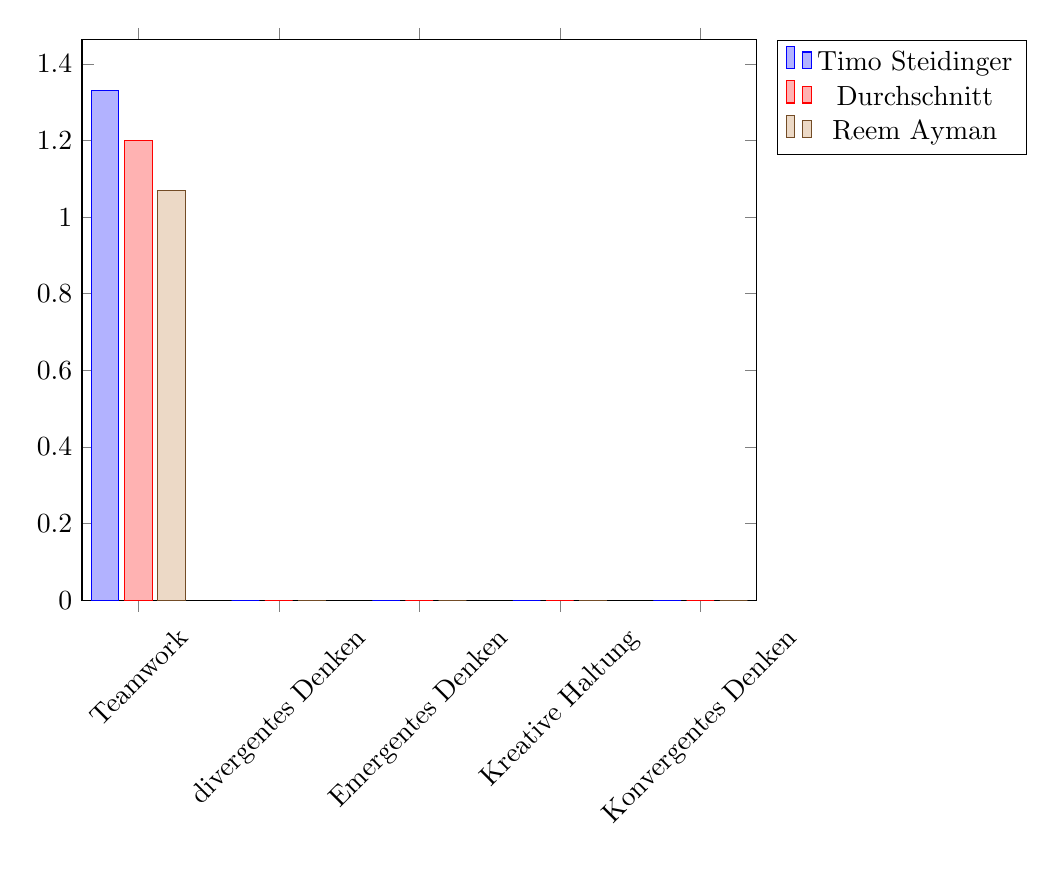
\begin{tikzpicture}
		\begin{axis}[
			ybar,legend pos=outer north east,ymin=0,scale = 1.25,
			symbolic x coords={Teamwork, divergentes Denken, Emergentes Denken, Kreative Haltung, Konvergentes Denken},
			xtick={Teamwork, divergentes Denken, Emergentes Denken, Kreative Haltung, Konvergentes Denken},
			xticklabel style={rotate=45}
			]
			%Timo
			\addplot coordinates
			{(Teamwork, 1.33)(divergentes Denken,0)(Emergentes Denken, 0)(Kreative Haltung, 0)(Konvergentes Denken,0)};
			%Durchschnitt
			\addplot coordinates
			{(Teamwork, 1.2)(divergentes Denken,0)(Emergentes Denken, 0)(Kreative Haltung, 0)(Konvergentes Denken,0)};
			%Reem
			\addplot coordinates
			{(Teamwork, 1.07)(divergentes Denken,0)(Emergentes Denken, 0)(Kreative Haltung, 0)(Konvergentes Denken,0)};

			
			\addlegendentry{Timo Steidinger}			
			\addlegendentry{Durchschnitt}
			\addlegendentry{Reem Ayman}

		\end{axis}
	\end{tikzpicture}

	\caption[Durchschnittliche Bewertung der Formulierungen]{Durchschnittliche Bewertung der Formulierungen zweier unabhängig voneinander bewertenden Person}
\end{figure}



\section{Entwicklung der Kinder}
\subsection{Jonas}
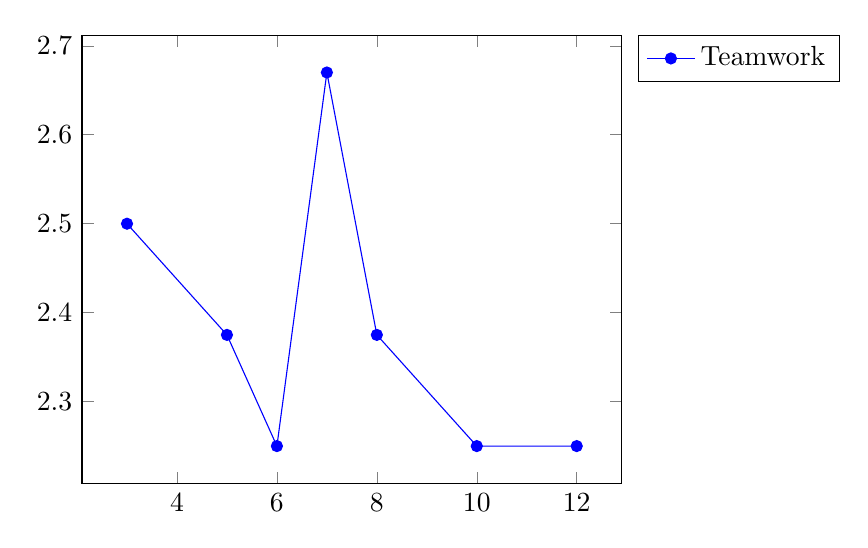
\begin{tikzpicture}
	\begin{axis}[legend pos=outer north east]
		\addplot[mark=*,blue]
		coordinates {
			(3,2.5) (5,2.375) (6,2.25) (7,2.67) (8,2.375) (10,2.25) (12,2.25)
		};
		\legend{Teamwork}
	\end{axis}
\end{tikzpicture}

\subsection{Mario}
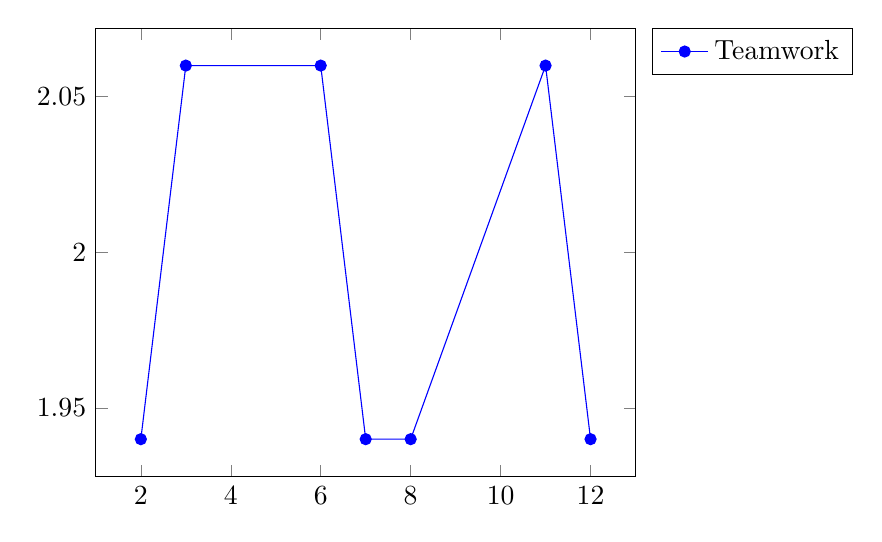
\begin{tikzpicture}
	\begin{axis}[legend pos=outer north east]
		\addplot[mark=*,blue]
		coordinates {
			(2,1.94)(3,2.06)(6,2.06)(7,1.94)(8,1.94)(11,2.06)(12,1.94)
		};
		\legend{Teamwork}
	\end{axis}
\end{tikzpicture}

\subsection{Sara}
\begin{tikzpicture}
	\begin{axis}[legend pos=outer north east]
		\addplot[mark=*,blue]
		coordinates {
			(3,.47) (5,.47) (6,.5) (7,.38) (8,0.93) (11,.88) (12,.93)
		};
		\legend{Teamwork}
	\end{axis}
\end{tikzpicture}


\subsection{Benny}
\begin{tikzpicture}
	\begin{axis}[legend pos=outer north east]
		\addplot[mark=*,blue]
		coordinates {
			(2,1.45)(3,1.31) (5,2.37) (6,2.06) (7,1.4) (8,1.33) (10,.57) (11,.5)(12,.54)
		};
		\legend{Teamwork}
	\end{axis}
\end{tikzpicture}


\subsection{Henriette}
\begin{tikzpicture}
	\begin{axis}[legend pos=outer north east]
		\addplot[mark=*,blue]
		coordinates {
			(2,2.21)(3,2)(5,2.31)(6,1.19)(7,1.75)(8,1.88)(10,1.79)(11,0.63)(12,0.63)
		};
		\legend{Teamwork}
	\end{axis}
\end{tikzpicture}

\subsection{Moritz}
\begin{tikzpicture}
	\begin{axis}[legend pos=outer north east]
		\addplot[mark=*,blue]
		coordinates {
			(2,2.43)(3,2.43)(5,1.5)(6,1.2)(10,1.33)(11,.73)(12,.53)
		};
		\legend{Teamwork}
	\end{axis}
\end{tikzpicture}


\subsection{Lulu}
\begin{tikzpicture}
	\begin{axis}[legend pos=outer north east]
		\addplot[mark=*,blue]
		coordinates {
			(2,2.01)(3,2.43)(5,1.14)(6,1.5)(7,1)(8,.67)(10,1)(11,.43)(12,.38)
		};
		\legend{Teamwork}
	\end{axis}
\end{tikzpicture}


\subsection{Heinz}
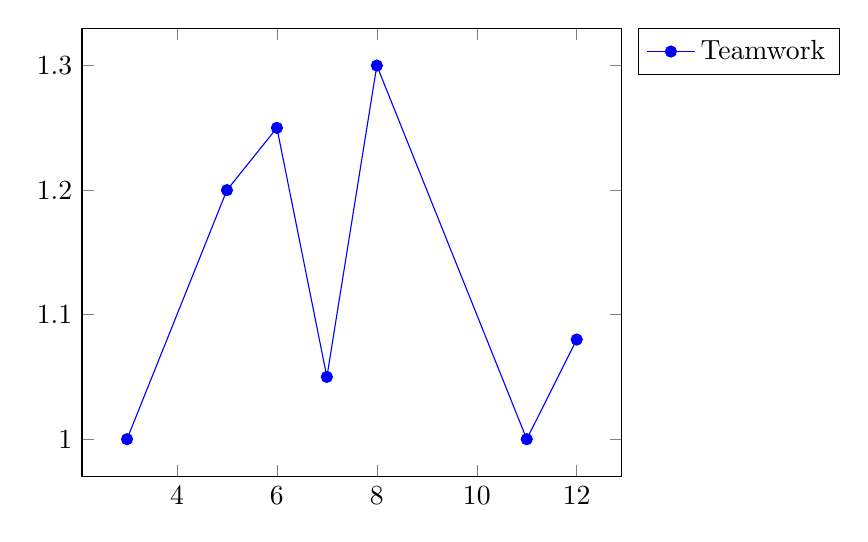
\begin{tikzpicture}
	\begin{axis}[legend pos=outer north east]
		\addplot[mark=*,blue]
		coordinates {
			(3,1)(5,1.2)(6,1.25)(7,1.05)(8,1.3)(11,1)(12,1.08)
		};
		\legend{Teamwork}
	\end{axis}
\end{tikzpicture}

\section{Persönlichkeitstypen und Entwicklung}
Liniendiagramm mit Termin auf X-Achse und Durchschnittswert der Persönlichkeitstypen auf Y-Achse


\subsection{Teamwork}
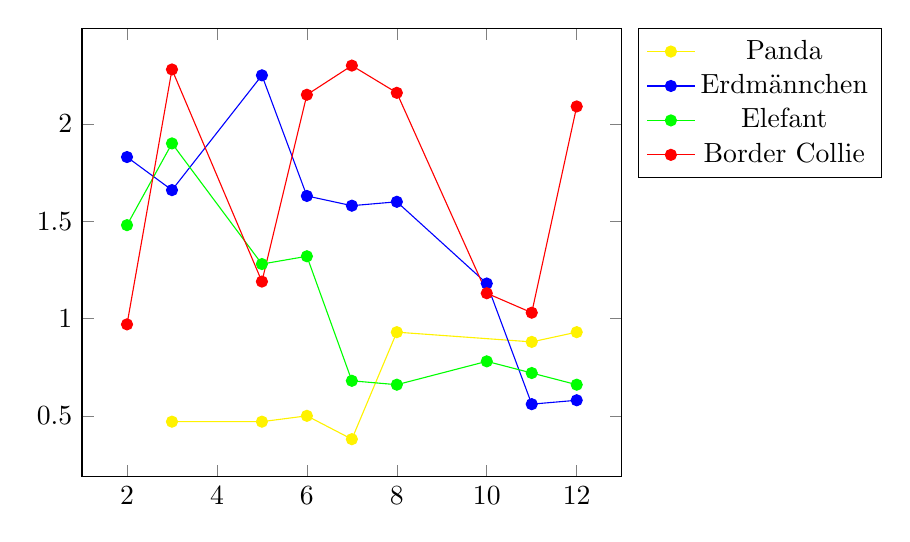
\begin{tikzpicture}
	
	\begin{axis}[legend pos=outer north east]
		\addplot[mark=*,yellow]
		coordinates {
			(3,.47) (5,.47) (6,.5) (7,.38) (8,0.93) (11,.88) (12,.93)
		};
		\addlegendentry{Panda}
		\addplot[mark=*,blue]
		coordinates {
			(2,1.83)(3,1.66)(5,2.25)(6,1.63)(7,1.58)(8,1.6)(10,1.18)(11,.56)(12,.58)
		};
		\addlegendentry{Erdmännchen}
		\addplot[mark=*,green]
		coordinates {
			(2,1.48)(3,1.9)(5,1.28)(6,1.32)(7,0.68)(8,0.66)(10,.78)(11,.72)(12,.66)
		};
		\addlegendentry{Elefant}
		\addplot[mark=*,red]
		coordinates {
			(2,.97)(3,2.28)(5,1.19)(6,2.15)(7,2.3)(8,2.16)(10,1.13)(11,1.03)(12,2.09)
		};
		\addlegendentry{Border Collie}
		
	\end{axis}
\end{tikzpicture}
\section{Computational Thinking Test}
	\subsection{Einordnung der Gruppe}
	
	\subsection{BCTt und CTt}